\section*{Appendix: Using the OIT Server}
If you wish to finish the Lab questions on the OIT server, please visit \url{https://vm-manage.oit.duke.edu/containers} and log into your Jupyter Notebook Environment. You can upload the files you need to the server by clicking the button shown in Figure~\ref{fig:upload}:
\begin{figure}[h]
\centering
  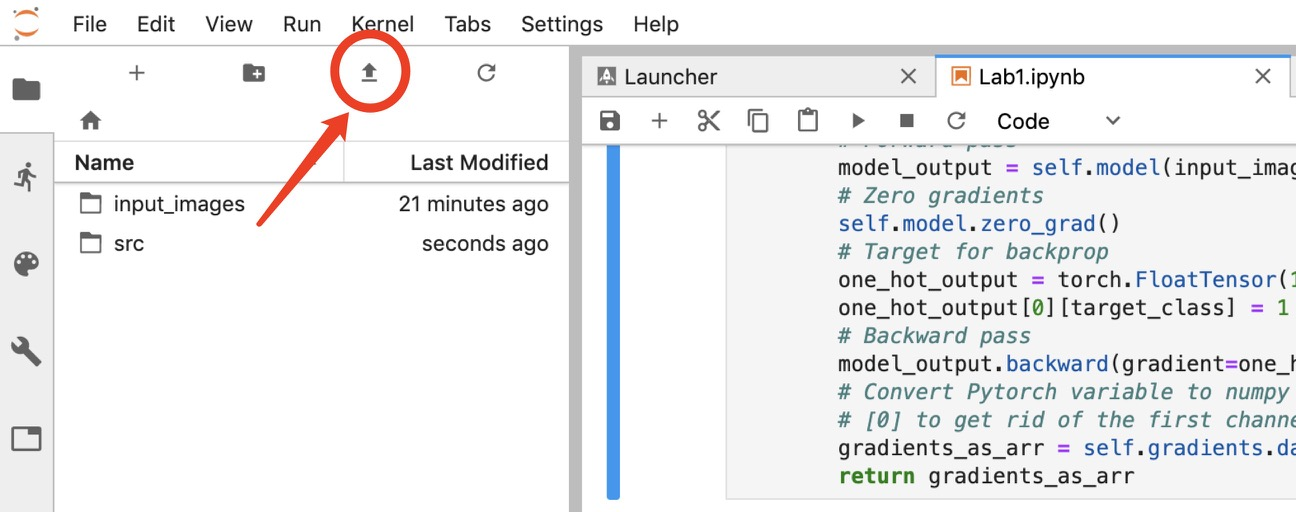
\includegraphics[width=0.8\linewidth]{upload_ins.jpg}
  \caption{Uploading files Instruction}
  \label{fig:upload}
\end{figure}

If you are uploading an zip file, you may unzip it on the server by:
\begin{itemize}
    \item Press the `$+$' button and click on ``terminal'' in the right-hand side ``Launcher'' column.
    \item In the terminal, type $unzip\ *.zip$
\end{itemize}
%After that, please use \texttt{LeNet5.ipynb} to start your first lab. Have fun!

\begin{warn}[Notice:]
After finishing the lab, please make sure you kill your current process by right-clicking on the \texttt{.ipynb} file and select ``Shutdown Kernel'', as shown in Figure~\ref{fig:shutdown}:

Please note that there is a 30-minute idle timeout for GPU access set on the OIT server. If you find that you can no longer access the GPU due to the timeout, simply save your progress, log out, restart your browser and log back in, then you can keep working again.
\end{warn}

\begin{figure}[h]
\centering
  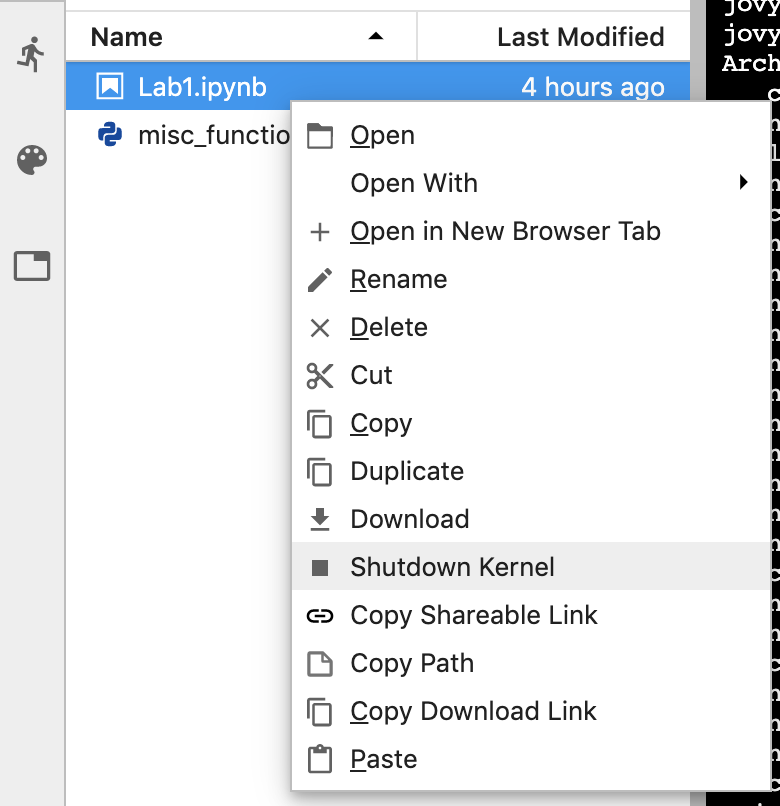
\includegraphics[width=0.3\linewidth]{shutdown.png}
  \caption{Shutdown kernel before exiting}
  \label{fig:shutdown}
\end{figure}
